\documentclass[class=scrartcl, crop=false]{standalone}
\usepackage[
typ={ohne},
fach=Informatik,
lerngruppe=SG-J1,
%loesungen=seite,
%lizenz={cc-by-nc-sa-4}
module={Aufgaben},
farbig
]{schule}
%\usepackage{polyglossia}
%\setmainlanguage{ngerman}
\usepackage[subpreambles=true]{standalone}
\usepackage{import}
\usepackage{fourier-otf}
\setmonofont{Ubuntu Mono Regular}[Scale=0.9]
\usepackage{shellesc}
\ShellEscape{pythontex \jobname.pytxcode }
\usepackage[
%prettyprinter=pygments, %pygopt={style=emacs}
]{pythontex}


\usepackage{hyperref}


\usepackage{booktabs}

\usepackage{minted}





\newcommand{\expandpyconc}[1]{\expandafter\reallyexpandpyconc\expandafter{#1}}
\newcommand{\reallyexpandpyconc}[1]{\pyconc{exec(compile(open('#1', 'rb').read(), '#1', 'exec'))}}

\newenvironment{pyconcodeblck}[1]
{\newcommand{\snippetfile}{snippet-#1.py}
	\VerbatimEnvironment
	\begin{VerbatimOut}{\snippetfile}}
	{\end{VerbatimOut}
	\expandpyconc{\snippetfile}}

\newcommand{\typesetcode}[1]{\inputpygments{python}{snippet-#1.py}}



\begin{document}

\begin{pyconcodeblck}{bedingte_ausführung}



def even_or_odd(number):
    if number % 2 == 0:
        return "Even"
    else:
        return "Odd"

def simple_multiplication(number) :
    if number % 2 == 0:
        return 8 * number 
    else:
        return 9 * number

def multiple(x):
    if x % 3 == 0 and x % 5 == 0:
        return "BangBoom"
    elif x % 3 == 0:
        return "Bang"
    elif x % 5 == 0:
        return "Boom"
    else:
        return "Miss"




def bool_to_word(boolean:bool):
    if boolean:
        return "Yes"
    else:
        return "No"

def bonus_time(salary, bonus):
    if bonus:
        return "$" + str(10 * salary)
    else:
        return "$" + str(salary)

def hoop_count(n):
    if n < 10:
        return "Keep at it until you get it"
    else:
        return "Great, now move on to tricks"


def rps(p1, p2):
    if p1 == p2:
        return "Draw!"
    if p1 == "rock" and p2 == "scissors" or p1 == "paper" and p2 == "rock" or p1 == "scissors" and p2 == "paper":
        return "Player 1 won!"
    else:
        return "Player 2 won!"


def paperwork(n, m):
    if n < 0 or m < 0:
        return 0
    else:
        return n * m


def avg(s1, s2, s3):
    return (s1 + s2 +s3)//3

def get_grade(s1, s2, s3):
    if avg(s1, s2, s3) >= 90:
        return "A"
    elif avg(s1, s2, s3) >= 80:
        return "B"
    elif avg(s1, s2, s3) >= 70:
        return "C"
    elif avg(s1, s2, s3) >= 60:
        return "D"
    else:
        return "F"



def basic_op(operator, value1, value2):
    if operator == '+':
        return value1 + value2
    elif operator == '-':
        return value1 - value2
    elif operator == '*':
        return value1 * value2
    else:
        return value1 / value2

\end{pyconcodeblck}

\section{Bedingte Ausführung}

\subsection{Zwei Alternativen}
\begin{aufgabe} \noindent
Implementiere eine Funktion \mintinline{python}{bool_to_word}, die ein \emph{Boolean} übergeben bekommt.
Wenn dieses \mintinline{python}{True} ist, soll \mintinline{python}{"Yes"} zurückgegeben werden. 
Wenn es \mintinline{python}{False} ist, wird \mintinline{python}{"No"} zurückgegeben. 

\begin{pyconsole}
bool_to_word(True)
bool_to_word(False)
\end{pyconsole}
	
\noindent\url{https://www.codewars.com/kata/53369039d7ab3ac506000467/train/python}
	
\end{aufgabe}
	

\begin{aufgabe} \noindent
Implementiere eine Funktion \mintinline{python}{hoop_count}, die dich motiviert Hulla-Hoop zu trainieren. Ihr wird die Anzahl der geschafften Drehungen übergeben. Wenn mehr als $10$ Umdrehungen geschafft wurden, gibt die Funktion \mintinline{python}{"Great, now move on to tricks"} zurück. Bei weniger als $10$ Umdrehungen soll \mintinline{python}{"Keep at it until you get it"} zurück gegeben werden.

\begin{pyconsole}
hoop_count(100)
hoop_count(1)
\end{pyconsole}

\noindent\url{https://www.codewars.com/kata/55cb632c1a5d7b3ad0000145/train/python}

\end{aufgabe}

\begin{aufgabe} \noindent
Deine Kollegen bitten dich darum ihnen Unterlagen zu kopieren.
Implementiere eine Funktion \mintinline{python}{paperwork}, die dir hilft die Anzahl der benötigten Seiten Papier zu berechnen. Der Funktion werden die Anzahl der Kollegen und die Anzahl der Seiten pro Kollege übergeben.
Wenn negative Zahlen übergeben werden, wurden fehlerhafte Daten übertragen. In diesem Fall soll \mintinline{python}{0} zurückgegeben werden.

\begin{pyconsole}
paperwork(3, 5)
paperwork(4, 6)
paperwork(-2, 60)
\end{pyconsole}

\noindent\url{https://www.codewars.com/kata/55f9b48403f6b87a7c0000bd/train/python}

\end{aufgabe}

\begin{aufgabe} \noindent
Implementiere eine Funktion \mintinline{python}{bonus_time}, die das Gesamtgehalt eines Mitarbeiters als String zurückgibt.
Die Funktion bekommt das Grundgehalt als \emph{Integer} und ein \emph{Boolean}, das angibt, ob der Mitarbeiter einen Bonus bekommt. Wenn dies der Fall ist bekommt der Mitarbeiter das zehnfache seines Grundgehalt. Ansonsten bekommt er nur das Grundgehalt.

\begin{pyconsole}
bonus_time(100, False)
bonus_time(50, True)
\end{pyconsole}
	
\noindent\url{https://www.codewars.com/kata/56f6ad906b88de513f000d96/train/python}


\end{aufgabe}


\subsection{Mehrere Alternativen}

\begin{aufgabe} \noindent
Implementiere eine Funktion \mintinline{python}{rps}, die genutzt werden kann um Schere-Stein-Papier zu spielen. Ihr werden die Entscheidungen der beiden Spieler übergeben und sie gibt zurück, wer gewonnen hat.

\begin{figure}[H]
	%\centerline{\includesvg[inkscapelatex=false,width=0.5\linewidth]{rock-paper-scissors}}
	\centering	
	
\includegraphics[width=0.4\linewidth]{rock-paper-scissors}
	\tiny \caption{\tiny \noindent\url{https://upload.wikimedia.org/wikipedia/commons/6/67/Rock-paper-scissors.svg}}
	%\label{fig: example}
\end{figure}

\begin{pyconsole}
rps("rock", "scissors")
rps("scissors", "paper")
rps("rock", "rock")
\end{pyconsole}
	
\noindent\url{https://www.codewars.com/kata/5672a98bdbdd995fad00000f/train/python}
	
\end{aufgabe}

\begin{aufgabe} \noindent
Implementiere eine Funktion \mintinline{python}{play_rps}. Mit dieser Funktion kann man zu zweit and der Konsole Schere-Stein-Papier spielen. Die Funktion fordert nacheinander die Spieler auf, sich für eine der drei Möglichkeiten zu entscheiden. Anschließend wird der Gewinner bekannt gegeben. Gehe davon aus, dass beide Spieler eine korrekte Eingabe eintippen.

\begin{figure}[H]
	%\centerline{\includesvg[inkscapelatex=false,width=0.5\linewidth]{rock-paper-scissors}}
\centering	
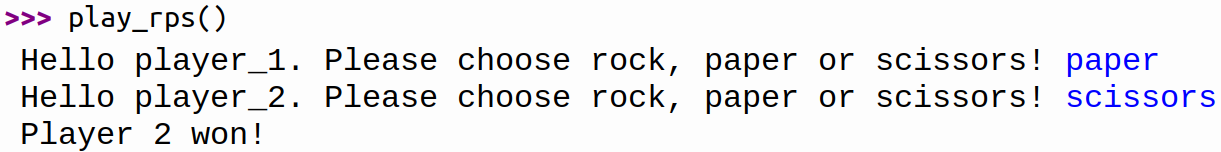
\includegraphics[width=\linewidth]{rps}
\end{figure}
\end{aufgabe}







%\begin{aufgabe} \noindent
%Implementiere eine Funktion \mintinline{python}{basic_op}, die als Taschenrechner genutzt werden kann. Der Funktion werden ein Symbol für eine Operation und zwei ganze Zahlen übergeben. Sie gibt das Ergebnis der Berechnung zurück.
%Bei den Beispielen unten sind alle möglichen Symbole für Operationen zu sehen.
%
%\begin{pyconsole}
%basic_op("+", 1, 2)
%basic_op("*", -3, -4)
%basic_op("-", 1, 2)
%basic_op("/", 10, 3)
%\end{pyconsole}
%	
%\noindent\url{https://www.codewars.com/kata/57356c55867b9b7a60000bd7/train/python}
%	
%\end{aufgabe}





\hinweis{Um die folgenden Aufgaben zu lösen, musst du dich mit der ganzzahligen Division auskennen}

\begin{aufgabe} \noindent
Implementiere eine Funktion \mintinline{python}{get_grade}, die einer Lehrerin an einer High-School hilft, die Noten in einem Schuljahr zu berechnen. Der Funktion werden die erzielten Punkte bei drei Klassenarbeiten übergeben. Sie gibt die erzielte Gesamtnote als String zurück. In jeder Arbeit konnten maximal $100$ Punkte erreicht werden.

\begin{table}[H]
\centering
	\begin{tabular}{ll} 
		\toprule
		Umrechnungstabelle \\  
		\midrule 
		Durchschnittliche Punktzahl & Note \\ 
		\midrule 
		$90 \leq \textnormal{Durchschnitt} \leq 100$ & A \\
		$80 \leq \textnormal{Durchschnitt} \leq 90$ & B \\
		$70 \leq \textnormal{Durchschnitt} \leq 80$ & C \\
		$60 \leq \textnormal{Durchschnitt} \leq 70$ & D \\
		$0 \leq  \textnormal{Durchschnitt} \le 60$ & F \\
		\bottomrule
	\end{tabular}
\end{table}

\begin{pyconsole}
get_grade(90, 91, 95)
get_grade(40, 60, 100)
get_grade(10, 50, 70)
\end{pyconsole}

	
\noindent\url{https://www.codewars.com/kata/55cbd4ba903825f7970000f5/train/python}
	
\end{aufgabe}


\begin{aufgabe} \noindent
Passe die Funktion \mintinline{python}{get_grade} so an, dass der Durchschnitt nur einmal berechnet wird.
\end{aufgabe}


\begin{aufgabe} \noindent
Implementiere eine Funktion \mintinline{python}{even_or_odd}, die eine ganze Zahl übergeben bekommt und \mintinline{python}{Even} zurückgibt, wenn diese Zahl gerade ist. Wenn die Zahl ungerade ist, soll \mintinline{python}{Odd} zurückgegeben werden. 
	
\begin{pyconsole}
even_or_odd(5)
even_or_odd(4)
\end{pyconsole}

\noindent\url{https://www.codewars.com/kata/53da3dbb4a5168369a0000fe/train/python}	

\end{aufgabe}

	
\begin{aufgabe} \noindent
Implementiere eine Funktion \mintinline{python}{simple_multiplication} die ein Integer übergeben bekommt.
Wenn dieses Integer gerade ist, gibt sie das achtfache zurück. Wenn es nicht gerade ist, gibt sie das neunfache zurück.
	
\begin{pyconsole}
simple_multiplication(2)
simple_multiplication(3)
\end{pyconsole}
	
\noindent\url{https://www.codewars.com/kata/583710ccaa6717322c000105/train/python}
	
\end{aufgabe}	
	
	
	

\begin{aufgabe} \noindent
Implementiere eine Funktion \mintinline{python}{multiple}, die ein Integer übergeben bekommt.
Wenn dieses Integer durch fünf und drei teilbar ist, gibt sie \mintinline{python}{"BangBoom"} zurück. 
Wenn das Integer durch fünf aber nicht durch drei teilbar ist, gibt sie \mintinline{python}{"Boom"} zurück.  Wenn es durch drei aber nicht durch fünf teilbar ist, gibt sie \mintinline{python}{"Bang"} zurück. Falls keine der Bedingungen erfüllt ist, so gibt sie   \mintinline{python}{"Miss"} zurück.
	
\begin{pyconsole}
multiple(2)
multiple(30)
multiple(20)
multiple(12)
\end{pyconsole}
	
\noindent\url{https://www.codewars.com/kata/55a8a36703fe4c45ed00005b/train/python}
	
\end{aufgabe}



\end{document}
